\documentclass[11pt]{article}

\usepackage{sectsty}
\usepackage{amssymb}
\usepackage{amsmath}
\usepackage{graphicx}
\usepackage{verbatim}
\usepackage{upquote}
\usepackage{longtable}
\newcommand{\tab}{\hspace*{2em}}
\includeonly{LRM}
\includeonly{tutorial}
\includeonly{white_paper}
\includeonly{logan}
\includeonly{nathan}
\includeonly{sid}
\includeonly{andrew}
\includeonly{justin}
\includeonly{conclusions}
\usepackage[margin=1.35in]{geometry}

\begin{document}

% title stuff
\title{DotPar \\ Final Report \\ Team 3}
\author{
Logan Donovan - lrd2127@columbia.edu \and
Justin Hines - jph2149@columbia.edu \and
Andrew Hitti - aah2147@columbia.edu \and
Nathan Hwang - nyh2105@columbia.edu \and
Sid Nair - ssn2114@columbia.edu}
\maketitle

%----------------------------
\part{Introduction}
\section{Motivation}
Moore's Law - the trend that the number of transistors that can fit on
a chip doubles every 2 years - has held true for half a century,
driving innovations in all areas of technology. But recently chip
manufacturers have moved away from ever-increasing clock speeds, the
usual manifestation of Moore's law, in favor of increasing the number of cores in CPUs to manage heat dissipation.

As consumer and business demands for speed grow, programs must now be
written differently in order to take advantage of multiple cores in order to utilize the
power of CPUs. However, the imperative programming paradigm that has prevailed in the programming community isn't conducive to safe,
parallel programming. Parallel programming is difficult and
synchronization bugs are notoriously difficult to fix.

Many solutions to this problem have emerged, but each has its drawbacks. We will
briefly survey some of the most prominent existing solutions.

\subsection{Locking}
Locking controls access to memory that is accessible by several threads of
execution. However, this requires that the programmer manually lock regions of code, which is both tedious and error prone. This can lead to deadlock and race conditions that are extremely
hard to debug.

\subsection{Task-based Concurrency and the Actor Model}
Task-based concurrency, used in languages like Ada and X10, doesn't
expose threads to the programmer. Simple computations, not threads, are
the unit of parallelization. The actor model, present in SmallTalk and
Scala, treats different threads as actors that communicate with each
other via message passing. Since the actors don't share state, this is
much less error prone than locking since race conditions can be
avoided entirely. These models can be elegant, but they still require
manual division of labor on the part of the programmer, which
introduces errors and overhead, especially when refactoring code. We
seek to avoid imposing this burden on programmers. Furthermore, they are
optimized for task-based parallelism when many of today's problems demand
data-based parallelism.

\subsection{Functional Programming}
The functional paradigm minimizes side effects in favor of
deterministic functions. Under this model, functions could easily be
parallelized because they execute independently. Functional languages
like Haskell boast compilers that produce a great degree of
parallelization.

However, the functional paradigm is an unfamiliar way of coding for
many programmers and having state is often a preferable way of
modeling a program. In particular, object-oriented approaches have
proven useful in building large applications. These factors have
limited the adoption of purely functional languages.

Additionally, the benefits of parallelizing a purely functional
programming languages is limited because objects must frequently
be copied as they are immutable. This means that cache hit rates
drop significantly, main memory bandwidth becomes a bottleneck, and
garbage collection becomes a pain\footnote{http://bit.ly/dotpar1}.

\subsection{Implicit Parallelization}
Some efforts to write implicitly parallel, imperative languages have
been made\footnote{See http://bit.ly/dotpar2 and http://bit.ly/dotpar3
  for examples.}. However, state- of-the-art compilers are not yet
capable of good implicit parallelization. While some cases of
potential parallelization are easy to recognize, many of them
difficult or impossible to find with static
analysis\footnote{http://bit.ly/dotpar4}.

With this in mind, implicit parallelization may sound daunting, but it
is important to remember that the compiler can miss many potential
opportunities for parallelization without sacrificing
performance. Even with a modest ability to find parallelization
opportunities, the performance of parallel programs is still limited
by the number of processors, not the number of threads that run
simultaneously. In fact, if too many threads are created, the overhead
of thread creation and execution will adversely affect performance.

% ------------------------------------------------------------
\section{Introducing DotPar}
With familiar C-like syntax, DotPar is a multi-paradigm language that
implicitly parallelizes code with minimal programming effort. By
abstracting parallelization, DotPar enables programmers to focus
on designing and and architecting systems instead of on micromanaging
performance. Additionally, it provides the expressive power of
functional languages and includes some imperative paradigms derived
from C to ease the job of the programmer.

\subsection{Automatic Parallelization}
Based on static analysis of code and user annotations, DotPar can
detect a large class of parallelization opportunities, speeding up
execution considerably.

\subsection{Strong Typing}
Keeping DotPar strongly typed provides compile-time
check for common mistakes that should never make it to
production. This also enhances the compiler’s ability to parallelize
the code.

\subsection{First-class Functions and Lexical Closures}
By providing first-class functions and closures, DotPar provides a
great degree of expressiveness not possible in a language like
Java. However, it is not as restrictive as a purely functional
language like Haskell because it provides some imperative constructs
as well.

\subsection{Robustness and Security}
Through implicit parallelization, DotPar removes the risk of race
conditions and deadlock.  And, since it runs on the JVM, the code is
robust and portable. Furthermore, DotPar raises informative
errors that allow the user to debug code efficiently and quickly,
reducing development time.

\subsection{Memory Management and Garbage Collection}
Since DotPar runs on the JVM, garbage collection and memory management
are handled automatically, reducing programmer overhead.


\part{Language Tutorial}
Parallel algorithms tend to be described as operations on collections of values.
For instance, ``find the minimum neighbor for each vertex'', or ``sum each row
of a matrix'' are data-centric operations that can be done in parallel.
\footnote{http://www.cs.cmu.edu/~scandal/cacm/node4.html} This ability to
operate in parallel over sets of data is often referred to as data-parallelism.
It is important that this data-parallelism can be exploited to its full
potential. We want to be able to run parallel functions in parallel to maximize
the efficiency of the program. Thus, we seek to provide an effective nested
data-parallel language.

The following tutorial will give a quick tour of the basics of the language and
build up to defining complex array manipulations to enable you to start writing
useful programs as soon as possible. To do that, we'll concentrate on the
basics: types, arithmetic expressions, arrays, control flow, functions, list
comprehensions, and some nifty built-in functions.

\section{Overview}
\subsection{Hello, World}
DotPar was designed with simplicity and power in mind. To illustrate this, let's
get started with a traditional ``Hello, World'' program that prints the words
``Hello, World'' to stdout.

\begin{verbatim}
func main:void()
{
    println("Hello, world!");
}
\end{verbatim}

Just like in C and Java, the DotPar execution begins with a function named
\verb=main=. Thus, every program must contain a main function. In this
\verb=main= method, we use the built-in function \verb=print= to print the
\verb=string= ``Hello, world''. A \verb=string= is an \verb=array= of
characters. We will explain exactly what \verb=function=s, \verb=string=s, and
\verb=char=s in later. But first, let's get this program running.

To compile and run this program there are three steps (assuming a UNIX-like
system). First, we should save the function in a file called
\verb=helloWorld.par=. DotPar programs are stored in files that have the
extension \verb=.par=. Next, we run a compiler on the program file, like so:

\begin{verbatim}
    dotparc helloWorld.par
\end{verbatim}

\verb=dotparc= can accept multiple files. So, to compile all the .par files in a
directory, you would run: 

\begin{verbatim}
    dotparc *.par
\end{verbatim}

If the program residing in the file has no syntax errors and is a complete
DotPar program then the compiler will produce an executable file:

\begin{verbatim}
    out.parc
\end{verbatim}

If there are errors during compilation those will be printed to your console. In
this example, running out.parc in the command line with:

\begin{verbatim}
    ./out.parc
\end{verbatim}

will produce the output:

\begin{verbatim}
    Hello, World
\end{verbatim}

We'll now walk you through some key features of the language. As you go along,
try writing and compiling these programs yourself.

\subsection{Types And Arithmetic Expressions}

DotPar contains the concept of types which are used to define a variable before
its use.  The definition of a variable will assign a store address for the
variable and define the type of data that will be held at that address.  DotPar
only three contains basic types: \verb=number=, \verb=boolean=, and \verb=char=.

\subsubsection{Numbers and Basic Arithmetic Operators}
All numbers in DotPar are double-precision 64-bit floating point numbers.  This
basic type is referred to as \verb=number=.  This simplicity allows for
computations to be straightforward while maintaining incredible precision. We
realized that since numbers were so imporant in the language that simplifying
everything to high precision and using the parallelization for performance gains
would make the language easier to use.

Our next program will illustrate the use of numbers and some basic arithmetic
expressions that can be used to manipulate numbers.

\begin{verbatim}
func main:void()
{
    number a = 1;
    number b = 2;
    println(b);
    println(a / b);
    number c = a + b;
    println(c);
}
\end{verbatim}

The first \verb=println= statement may be counterintuitive to what one might
expect.  This statement will not return \verb=2=, but rather \verb=2.0=.
Following this logic, the second print statement should, and does return
\verb=.5=.  The last print statement's output should now be obvious as
\verb=3.0=.

Other basic arithmetic operators include \verb=-= , \verb=*=, and \verb=/= which
represent subtraction, multiplication, and division, respectively.  There is
also a remainder operator, \verb=\%=,  which returns the remainder of the
division of two numbers.

Note: \verb=+,= \verb=-,= \verb=*,= \verb=/,= \verb=sqrt,= \verb=ln,=
\verb=log(num, base),= \verb=exp(num, exponent),= \verb=ceil,= \verb=floor,=
\verb=trunc,= \verb=round,= \verb=sin(x),= \verb=cos(x),= \verb=tan(x),=
\verb=asin(x),= \verb=acos(x),= \verb=atan(x)= are all supported. The
trigonometric functions return a value in radians, and the inverse trigonometric
functions expect a value in radians.

\subsubsection{Booleans and Operators}
The boolean data type has only two possible values, \verb=true= and
\verb=false=.  This uses simple flags that track true/false conditions. While
this data type represents one bit of information, but it is treated internally
as a 32-bit entity. We decided to have booleans because they are a very useful
data type. We implemented them as 32-bit entities because that is how Java does
it.

The following program will give an elementary example of the use of booleans, and their uses.  

\begin{verbatim}
func main:void()
{
    boolean b = true;
    println(!b);
    boolean c = false;
    println(b && c);
    println(c || b);  
}
\end{verbatim}

Since a boolean tracks a single true/false condition, each print statement will
only return either \verb=true= or \verb=false=.  The ! symbol is the NOT unary
operator and evaluates to the complement of its argument.  Since \verb=b= is
\verb=true=, the first print statement will be ``\verb=false=''.  The \verb=&&=
operator signifies the binary operator AND which returns the conjunction of its
two arguments.  So the second print statement will return false, since true AND
false evaluates to false. The \verb=||= operator signifies the binary operator
OR which returns the disjunction of its two operators.  So the last print
statement will return true, since false OR true evaluates to true. 

\subsubsection{Char}
The char data type is a single 16-bit Unicode character. 

The following example will given an elementary example of the use of chars.

\begin{verbatim}
func main:void()
{
    char c = 'a';
    println(c);
}
\end{verbatim}

The above will print out ``a'', without the quotations. Often chars by
themselves are not very useful, as in reality we use a sequence of chars to
represent words, or strings.  This provides a nice transition to DotPar's
arrays.

\subsection{Arrays and Control Flow}
There are times when writing programs when you may want to store multiple items
of same type together. Arrays provide this functionality. They are contiguous
bytes in memory, which facilitates easy searching and manipulation of lists of
elements. Like everything else in the language, arrays are typed. You can have
an array of any type, such as \verb=number=, \verb=boolean=, \verb=char=, or
another array. Let's take a look at some examples.

\subsubsection{Revisiting Hello, World}

\begin{verbatim}
func main:void()
{
    char[] helloWorld = "Hello, World";
    println(helloWorld);
}
\end{verbatim}

The first program we learned to write prints the words ``Hello, World.''  In this equivalent program, we explicitly create an array of type \verb=char= in the first line of \verb=main=. An arrays of chars is also often called a \verb=string=. Arrays are very fundamental building blocks in DotPar. Rather than have many built-in types, DotPar has just a few types and gives users the power to create more complicated types. So, there is no built-in \verb=string= type, so there is instead only an arrays of characters. So, the first line creates a character array with each element being a character in the statement, ``Hello, World''.

Arrays are where DotPar leverages its power as it can manipulate large sets of data quickly by manipulating arrays, iterating through arrays, and applying functions to arrays. 

\subsection{Array Iteration}
\subsubsection{the each method}
Our next example program creates an array of type number and demonstrates a
method of iterating through an array. The first line creates an array arr of
size 10 and populates it with the numbers 1-10. Notice at the end of the line
there is a \verb=//=. This is a single-line comment. \verb=//= will cause the
compiler to ignore the rest of the line. Comments are a useful to markup text to
explain subtleties of the code. They are ignored by the compiler, so they are
not evaluated. The second line demonstrates the use of the built-in \verb=each=
function, which is used to iterate over an array element by element. For each
loops contain all of its statements within curly brackets.  This for each
iterates through every number in arr and calls the function print on every
element. This prints a list of the elements in arr to standard out.

\begin{verbatim}
func main:void()
{
    number[] arr = [1,2,3,4,5,6,7,8,9,10];  //create the array
    each(arr, func:void(number n) { println(n); });
}
\end{verbatim}

\subsubsection{the for loop}
Another way to write the program above would be to use a \verb=for= loop, which can be used to iterated over the indices of an array by using a counter. So, the variable \verb=i= of type number is created and is initialized to 0. It then checks to ensure that \verb=i= is less than \verb=len(arr)=. \verb=len= is an example of a built-in function that returns a \verb=number= whose value is the length of the array in its argument. In \verb=for= loop we are again calling the \verb=print= function and are passing in \verb=arr[i]=, which is the value in the array at index \verb=i=. The \verb=for= loop then lastly increments \verb=i= by 1.

\begin{verbatim}
func main:void()
{
    number[] arr = [1,2,3,4,5,6,7,8,9,10];
    number i;
    for(i = 0; i < len(arr); i = i + 1) {
        println(arr[i]);
    }
}
\end{verbatim}

Arrays can be extended to arbitrarily many dimensions. For example, we create a matrix in the example below.

\begin{verbatim}
func main:void()
{
    number[][] matrix = [ [1,2,3], [4,5,6], [7,8,9] ];
    println(matrix);
}
\end{verbatim}

Here we are creating a two-dimensional \verb=3x3= array with the numbers 1 through 9.  We have a  set of \verb=[ ]= for each dimension we want create.  We can fill this array with nested brackets by defining each row within brackets. Try running this program and see what it prints!

\subsection{Control Statements}

Next, we'll look at conditional statements, random number generation, and the fill statement in DotPar. 

Let's take a look at our next example program.

\begin{verbatim}
func main:void()
{
    /*
    This program creates an array of length 10 and 
    fills it with random numbers in the range [0-100).
    It then prints out each element with 
    a message declaring it even or odd.  
    */

    number[] arr;
    fill(arr, func:number(number index) { return rand(100); }, 10);
    char[] even = “is even”;
    char[] odd = “is odd”;

    each(arr, func:void(number element) {
        if (element % 2 == 0) {
            println(element + “ “ + even);
        } else {
            println(element + “ “ + odd);
        }
    });
}
\end{verbatim}

First, notice that the first few lines of the function demonstrate another way to comment in DotPar by using traditional C style comments, \verb=/* ... */= to comment out an entire block of text.

Next, we create an number array arr. The next line calls the built-in function \verb=fill(array, function)= which takes in an array and a function as arguments and inserts values into the array according to the passed in function. In this case we are passing in the \verb=rand(number)= function. \verb=rand= generates random numbers in the range [0, cap). Afterwards, we create two character arrays that contain the text ``is even'' and `` is odd'' which will be used later.

Next we have a call to our old friend, the \verb=each= function, that iterates through each element in the array. Within the body of the \verb=each= function we have our first example of \verb=if= statements in DotPar. They follow the form: 

\begin{verbatim}
if (conditional) {
   // code
} elif (conditional) {
   // code
} else {
   // code
}
\end{verbatim}

There must be exactly one \verb=if= clause, any number of \verb=elif= clauses, and no more than one \verb=else= clause.

The parenthetical after the \verb=if= is the condition that must be met in order to run the code within the braces. If this condition is true, the code with the braces of the else is run. The conditional we test for in this example is \verb=element \% 2 == 0=. \verb=element= is the value in the array, the \verb=\%= is the arithmetic operation for modulus, the \begin{verbatim}== 
\end{verbatim} tests equality, and 0 is the number 0. Within the \verb=if= we print the number followed by the character sequence specifying it is even and within the \verb=else= we print the number followed by the character sequence specifying it is odd.

\subsection{List Comprehensions}
As a more complicated example, you may want to write something like:

\begin{verbatim}
    number[] foo = [1,2,3,4,5];
    number[] squares;
    number i;
    for(i = 0; i < len(squares) ; i = i + 1){
        if (squares[i] % 2 == 0) {
            squares[i] = exp(foo[i], 2);
        }
    }
\end{verbatim}

This function creates an array with the square of the even numbers in the original array. But this is rather verbose, which seems unnecessary for a conceptually simple task like this. DotPar provides an easy way to express this logic, borrowing the useful list comprehension from Python and Haskell. We will illustrate the power of list comprehensions by replacing the previous program fragment in one line:

\begin{verbatim}
number[] squares = [exp(x,2) for number x in [1,2,3,4,5] if (x % 2 == 0)];
\end{verbatim}

You can also use an expanded notation for using n arrays, such as

\begin{verbatim}
number[] foo = [x*y for number x, number y in [1, 3, 9], [1, 2, 3] if (x != 1)];
\end{verbatim}

\subsection{Working with Functions}
In DotPar, functions are first-class, which means they can be assigned to variables or passed to other functions as arguments. A function provides a convenient way to encapsulate some computation, which can then be used without stressing its implementation. All functions are declared with the \verb=func= reserved word, and can be nested within each other.

A function definition has this form:

\begin{verbatim}
func function-name : return-type(optional parameter declarations)
{
    declarations and statements;
    return return-val;
}
\end{verbatim}

\subsubsection{Revisiting main}
With this in mind, let's take a look at \verb=main= again. As in Java, \verb=main= can accept arguments. However, as in C, the arguments can be omitted.

\begin{verbatim}
func main: void(char[][] args)
{
    if (len(args) > 0) {
      each(args, func: void(char[] s) { println(s); });
    }   
    else {
      println(“No arguments passed!”);
    }
}
\end{verbatim}

Try running this program, passing various arguments and check out the results.

\subsubsection{Declaring an Array}
Next, let's fill a create a matrix of integers. This example will demonstrate how to pass functions as parameters.

\begin{verbatim}
func main: void()
{
// This creates an array with 10 rows and 20 columns. The values are not populated,
// so they are random.
    number[10][20] b;
}
\end{verbatim}

\subsection{Idioms and Parallelism}
Our next sample programs will contain more complex array manipulation and introduce some useful functions for arrays. These functions aren't common in imperative languages, and they exhibit some nice properties of DotPar.

\subsubsection{Map}
\verb=map(array, function)= calls \verb=function(item)= for each of the array's items and returns an array of the return values.  For example, let's compute some cubes:

\begin{verbatim}
func main:void(){
    func cube:number (number value, number index){
        return value*value*value;
    }
    number[] a = [1,2,3,4,5];
    map(a, cube);
}
\end{verbatim}

Note that this example could have been computed more succinctly with a list comprehension. However, in some cases, you may find a \verb=map(array, function)= to be clearer. When you run map it returns a transformed list. Whereas when you run each it performs the functions and returns nothing, instead usings the 

\subsubsection{Reduce}
\verb=reduce(array, function, original)= returns a single value constructed by applying the reducing function repeatedly to the reduced value so far and each element of the array. For instance, if you wanted to add all the elements of a numerical array, one could define the function \verb=sum(number a, number b)=, and apply \verb=sum= to the array.

To break things down, we take the first two elements of the array and apply \verb=sum= to them. This returns the sum of the elements, our first result. Then, we take the third element of the array, and apply \verb=sum= to our first result and the third element, obtaining our second result. We continue in this manner, until we have one result and no more elements to reduce.

For a concrete example, let's compute the sum of the numbers 1 to 10000:

\begin{verbatim}
func main:void(){
   func sum:number (number a, number b){
       return a+b;
   }
   number[] x;
   fill(x, func:number(number index) { return index+1; }, 10000);
   // 0 is the starting value, we do this so that we can return 0 
   //if the array is  empty
   //Here we are filling the array with the values 0 - 10000 for 
   //the use in the suming function
   println(reduce(x, sum, 0));
}
\end{verbatim}

\subsubsection{Matrix Multiplication}
In this example we introduce nested functions and explore how working with functions can create clearer and better code. We'll also take a look at the feature that gives DotPar its name: implicit parallelism.

\begin{verbatim}
func matrixMultiply:number[][](number[][] a, number[][] b) {
    func transpose: number[][](number[][] a) {
        number[len(a[0])][len(a)] transposed;
        number i;
        number j;
        for (i<0; i < len(a); i = i + 1){
            for (j<0; j < len(a[0]); j = j+ 1){
                transposed[j][i] = a[i][j];
            }
        }
        return transposed;
    }

    func sum:number(number a, number b) {
          return a + b;
    }
    
    func dotprod:number(number[] a, number[] b) {
          return reduce([x * y for number x, number y in a, b], sum );
    }
    
    if (len(a) != len(b[0])) {
          return nil; // one can always return nil in place of a real value
    }
    
    return [[dotprod(row, col) for number[] col in transpose(b)] for number[] row in a];
}
\end{verbatim}

The function \verb=transpose= returns a transpose of the input matrix. The
function \verb=matrixMultiply= takes in arguments which are two two-dimensional
arrays, \verb=a= and \verb=b=. The function \verb=dotprod= accepts two
one-dimensional arrays and calls the reduce function, which calls the sum
function on each \verb=x=, \verb=y= pair which are elements in arrays \verb=a=
and \verb=b=. The final line returns a statement that pairs every row in
\verb=a= with every column in \verb=b= and calls the function \verb=dotprod=.

\subsubsection{Parallelization}
These examples demonstrate the power of DotPar's implicit parallelization.

The \verb=map= and \verb=reduce= functions can be parallelized, given certain
restrictions. If the functions only access variables passed to them and do not
mutate outside state, the mappings and reductions can be automatically
parallelized and executed on multiple cores. For instance, the computation done
by \verb=map= and \verb=reduce= can be done in $O(n/m)$ time, where $n$ is the
size of the array and $m$ the number of processors. In the transpose function
from the previous section, each cell in the new matrix can be computed
independently of the other, so DotPar will parallelize this multiplication if it
is appropriate given the computer's architecture and the nature of the
computation.

\section{Conclusion}
In this tutorial we have covered compiling your programs and writing basic
assignment and logical statements all the way through to more complicated
features like map, reduce, list comprehensions, and nested functions. With all
of the these tools now available, you should now be able to unleash the
performance power that DotPar provides for data manipulation.


\part{Language Reference Manual}
DotPar is a flexible language that provides implicit nested data parallelism with powerful first-class functions while providing a familiar imperative interface. The focus is on parallel performance for arrays and loops, since these are often the source of performance bottlenecks.
\\ \\*Previous implementations of nested data-parallel languages have relied on the use of purely functional paradigms which can make the learning-curve steep and difficult to those who just want to pick up a new tool. DotPar provides a multi-paradigm nested data-parallel language with a friendly imperative style in addition to powerful functions. Its implicit parallelism focuses on the performance of arrays and loops, but its implementation requirements are flexible enough for other forms of parallelism as well.

\section{Lexical Convention}
A program consists of zero or more input statements, and one or more lines stored in files. These are translated in several phases, which are described in Section 13. The first phases do low-level lexical transformations, which reduce the program to a series of tokens.

\tab \emph{lines:} 
\\* \tab \tab \tab \textit{imports\_opt external\_declaration}
\\* \tab \tab \tab \emph{lines external\_declaration}

 \tab \emph{imports:}
\\* \tab \tab \tab \textit{imports import\_declaration}
\\* \tab \tab \tab \textit{import\_declaration}

import\_declarations will be explained in detail in Section 11.

\section{Tokens}
DotPar has 5 token classes: identifiers, keywords, literals, operators, and other separators. All white space, collectively including blanks, horizontal and vertical tabs, newlines, and comments as described below are ignored except as they separate certain tokens. Sometimes white space is required to separate otherwise adjacent identifiers, keywords, and literals.
\subsection{Comments}
The characters /* introduce a block comment, which terminates with the characters */. In addition, // adds line comments which converts everything that follows to a comment until the end of the line. Comments do not nest, and they do not occur within string or character literals.
\subsection{Constants}
Constants are character, number, or string literals, as well as true, false, or nil.
\\ \emph{constant}
\begin{itemize}
\item
CHAR\_LITERAL
\item
NUM\_LITERAL
\item
STRING\_LITERAL
\item
TRUE
\item
FALSE
\item
NIL
\end{itemize}
\subsubsection{Character Literal}
A character constant specifies a single ascii character surrounded by single quotes, such as `a'. If one is so inclined, he or she can include such control characters as newlines by using traditional backslash delimited escape codes. For instance, a newline is `\textbackslash n', and `\textbackslash 0' is the null character. A notable exception is the backslash itself, which is merely `\textbackslash'.
\\ \\* A char literal has the type char and is initialized with the given ascii character. The behavior of a program that attempts to alter a char literal is undefined.
\subsubsection{Number Literal}
There are two ways to represent literal numbers with DotPar: the first is an integral format, without a decimal point, and the second is a floating point representation, including a decimal point.
\\ \\* The integral representation is merely a series of digits without spaces between them, like 31 or 42. Integral number literals are only available for base 10.
\\ \\* The floating point representation is a series of digits with a period embedded within or prepended to the front, and without spaces anywhere. Examples include 3.14159, or .11235, but not 125. with a trailing period.
\\ \\* The floating point representation is restricted to base 10, and there is no support for scientific notation.
\\ \\* A number literal has a type number and is initialized with the given value: if the given literal is too large, the behavior of the program will be undefined.
\subsubsection{String Constant}
A string literal is a sequence of ascii characters surrounded by double quotes as in ``. . . ''. A string has type `array of characters' and is initialized with the given characters. One may include traditional backslash escape codes, similar to character constants explained above. The behavior of a program that attempts to alter a string literal is undefined.
\subsubsection{Boolean Constant}
There are only two values for a boolean constant, \verb!true! or \verb!false!. Their literal value is respectively represented as \verb!true! and \verb!false!, not decorated by any special characters.
\subsubsection{Nil Constant}
\verb!nil! is a special literal that can stand in for any other type of value. \verb!nil! evaluates to \verb!false!. \verb!nil! and \verb!false! are the only values in the language that evaluate to \verb!false!.
\subsection{Identifiers}
An identifier is a sequence of letters and digits, and underscores. The first character must be a letter. Identifiers are case-sensitive and may have any length.
\subsection{Keywords}
The following identifiers are reserved for use as keywords, and may not be used otherwise:
\begin{itemize}
\item
\verb!import!
\item
\verb!true!
\item
\verb!false!
\item
\verb!boolean!
\item
\verb!char!
\item
\verb!func!
\item
\verb!number!
\item
\verb!void!
\item
\verb!if!
\item
\verb!else!
\item
\verb!elif!
\item
\verb!for!
\item
\verb!in!
\item
\verb!return!
\end{itemize}

\section{Syntax Notation}
The syntax in this manual has categories written in italics and literals and characters in
plain font. Optional terminal and nonterminal symbols have the subscript ``opt,'' like below:

\centerline{\{expression\_opt\}}

*An non-terminal with the name foo\_opt will either go to ``the empty string'' or foo. Similarly, lists follow the format of imports above. To avoid repetition, rules that follow this rigid structure will not be explained in-depth. However, they will be included in the complete grammar at the end of this reference manual.
\section{Meaning of Identifiers}
Identifiers are simply the names given to functions and variables. A variable is used to store data and points to a specific location. The interpretation of the data is based on the variable's type. Identifiers are limited to the scope within which they are defined and are only accessible within that scope. This can be only within a specific function or an entire program.
\\All variables declared are initialized to a default value: number = 0, boolean = false, char = ``'', number[] = [].
\subsection{Basic Types}
DotPar contains three basic types: number, boolean and char. Variables of type number are 64-bit double precision floating point numbers. Boolean variables have only two possible values: true and false. They are internally treated as a 32-bit entities. Char variables can store any member of the set of characters. Every character has its value as equivalent to the integer code for the character.
\subsection{Derived Types}
These include arrays and functions which can be constructed from the basic types. Derived types include:
\begin{itemize}
\item
\emph{arrays} of elements of a given type
\item
\emph{functions} accepting variables of certain types, and returning variables of a given type
\end{itemize}
There are infinitely many derived types. Type declaration syntax are described in more detail below.

\section{Objects and lvalues}
A variable is a named region of storage and an lvalue is an expression referring to that variable. For example, an lvalue expression can be an identifier with a specified type. Like in C, the term ``lvalue'' originates from the term left-value which indicates that it was on the left side of the assignment operator. Each operator listed below can expect lvalue operands and yields an lvalue.

\section{Expressions}
The precedence of expression operators is the same as the order of the major subsections outlined below in this section, with highest precedence first. In all subsections, precedence follows C-style conventions.  Left- or right-associativity is specified in each subsection for the operators discussed therein. The grammar given in Section 13 incorporates the precedence and associativity of the operators.
\\ \\*The precedence and associativity of the operators is fully specified, but the order of evaluation of expressions is undefined, even if the subexpressions involve side effects. However, each operator combines the values it produces by its operands in a way that is compatible with the parsing of the containing expression in which it appears. The handling of overflow, divide check, and other exceptions in expression evaluation is undefined by the language spec.
\subsection{Primary Expressions}
Primary expressions are identifiers, constants, string literals, or expressions in parentheses.
\\ \\* \tab \emph{primary\_expression:}
\\* \tab \tab \emph{IDENTIFIER}
\\* \tab \tab \emph{constant}
\\* \tab \tab \emph{(expression)}
\\ \\* An identifier is a primary expression. Its type is specified by its declaration, which must occur earlier in the program.
\\ \\* A constant is a primary expression. Its type depends on its form as discussed in section 2.2
\\ \\* A string literal is a primary expression. It is actually converted to an array of characters, but string literals are included as part of the grammar for programmer convenience.    
\\ \\* A parenthesized expression is a primary expression whose type and value are identical to those of the unadorned expression. 

\subsection{Postfix Expressions}
The operators in postfix expressions group left to right.
\\ \\* \tab \emph{postfix\_expression:}
\\* \tab \tab \emph{primary expression}
\\* \tab \tab \emph{postfix\_expression [ expression ]}
\\* \tab \tab \emph{postfix\_expression ( argument\_expression\_list\_pt)}
\subsubsection{Array References}
A postfix expression followed by an expression in square brackets is a postfix expression denoting a subscripted array reference. The postfix expression must evaluate to an array and the expression must evaluate to a type number.
\subsubsection{Function call}
A postfix expression followed by the function designator, followed by parentheses containing a possibly empty, comma-separated list of assignment expressions, which constitute the arguments to the given function.   
\\ \\* The term argument is used for an expression passed by a function call; the term parameter is used for an input object (or its identifier) received by a function definition, or described in function declaration. The scope is lexical.
\\ \\* Arguments are passed by value. A function may change the values of its parameter objects, which are copies of the argument expressions, but these changes cannot affect the values of the arguments. 
\\ \\*However, array references are passed by value, so a function may modify the contents of an array passed to it. 
\\ \\* Type agreement is strict between the parameters and arguments. Thus, DotPar is strongly and statically typed.          
\\ \\* The order of evaluation of arguments is unspecified. In addition, the arguments and their side effects need not be fully evaluated before the function is entered if the compiler can guarantee that this does not affect the correctness of the program. 

\subsection{Unary Expressions}
Expressions with unary operators group right-to-left.
\\ \\* \tab \emph{unary\_experession:}
\\* \tab \tab \emph{postfix\_expression}
\\* \tab \tab \emph{NOT unary\_expression}
\\* \tab \tab \emph{SUB unary\_expression}
\\ \\* The NOT unary\_expresssion refers to the ! operator. The operand of the ! operator must have a boolean type, and the result is true if the value of its operand evaluates to false, and false otherwise. The type of the result is boolean.
\\ \\* The SUB unary\_expression refers to the - operator. The operand of the - operator must have a number type, and the result is the negation of the value of its operand. The type of the result is number.

\subsection{Arithmetic Expressions}
Arithmetic Expressions are grouped left to right, and include: \%, /, *, + , - but this is infact is not useful, as it is parsed to preserve C style precedence. All operators return number types.
\\ \\* \tab \emph{arithmetic\_expression:}
\\* \tab \tab \emph{unary\_expression}
\\* \tab \tab \emph{arithmetic\_expression REM arithmetic\_expression}
\\* \tab \tab \emph{arithmetic\_expression DIV arithmetic\_expression}
\\* \tab \tab \emph{arithmetic\_expression MULT arithmetic\_expression}
\\* \tab \tab \emph{arithmetic\_expression ADD arithmetic\_expression}
\\* \tab \tab \emph{arithmetic\_expression SUB arithmetic\_expression}
\\ \\*REM refers to the \% operator, the remainder which refers to the remaining value after quotient the first operand by the second. Note that the remainder of a negative value will be negative.
\\ \\*DIV refers to the / operator, the division which refers to quotient of the first operand and the second.
\\ \\*MULT refers to the * operator, the multiplication between its two operands.
\\ \\*ADD refers to the + operator, the addition between its two operands.
\\ \\*SUB refers to the binary - operator, the subtraction between its two operands.

\subsection{Relational Expressions}
The relational operators group left-to-right.
\\ \\* \tab \emph{relational\_expression:}
\\* \tab \tab \emph{arithmetic\_expression}
\\* \tab \tab \emph{relational\_expression GEQ relational\_expression}
\\* \tab \tab \emph{relational\_expression GT relational\_expression}
\\* \tab \tab \emph{relational\_expression LT relational\_expression}
\\* \tab \tab \emph{relational\_expression LEQ relational\_expression}
\\* \tab \tab \emph{relational\_expression EQ relational\_expression}
\\* \tab \tab \emph{relational\_expression NEQ relational\_expression}
\\ \\* The GEQ refers to \textgreater= operators(greater or equal), GT to \textgreater (greater), LT to \textless (less than), LEQ to \textless= (less than or equal), EQ to == (equality), and NEQ to != (not equality). All yield false if the specified relation is false, and true if it is true. The type of the result is boolean. The usual arithmetic conversions are performed on arithmetic operands. GEQ, GT, LEQ, and LT have higher precedence than EQ and NEQ.

\subsection{Conditional Expressions}
The conditional operators group left-to-right and include \&\& and \textbar\textbar.
\\ \\* \tab \emph{conditional\_expression:}
\\* \tab \tab \emph{relational\_expression}
\\* \tab \tab \emph{conditional\_expression OR conditional\_expression}
\\* \tab \tab \emph{conditional\_expression AND conditional\_expression}
\\ \\*OR refers to the \textbar\textbar operator which performs a logical OR on its two operands which must be of type boolean. The result is of type boolean. 
\\ \\*AND refers to the \&\& operator which performs a logical AND on its two operands which must be of type boolean. The result is of type boolean.

\subsection{Array Expressions}
Array Expressions are conditional statements, or list\_comprehnesionsand initializer\_list\_opt enclosed in square brackets `[' ,`]'.
\\ \\* \tab \emph{array\_expression:}
\\* \tab \tab \emph{conditional\_expression}
\\* \tab \tab \emph{[ list\_comprehension ]}
\\* \tab \tab \emph{[ initializer\_list\_opt ]}
\\ \\*An initializer\_list is used in the creation of array literals.
\subsection{List Comprehension}
*List comprehensions are used to succinctly create an array. They are equivalent in power to maps and filters, but are often a more convenient syntax to use. Although the list comprehension may be parallelized during its execution, the ordering of the resulting array is deterministic.
\\ \\* \tab \emph{list\_comprehension:}
\\* \tab \tab \emph{array\_expression FOR paren\_parameter\_list\_opt IN array\_expression if\_comp\_opt}
\\* \tab \tab \emph{array\_expression FOR paren\_parameter\_list\_opt IN                               paren\_multi\_array\_expression\_list\_opt if\_comp\_opt}
\\ \\* The list comprehension syntax and behavior is very similar to Python's.

\subsection{Assignment Expressions}
There is one assignment operator =, and it is not used more than once per statement.
\\ \\* \tab \emph{assignment\_expression: }
\\* \tab \tab \emph{array\_expression}
\\* \tab \tab \emph{anonymous\_function\_definition}
\\* \tab \tab \emph{postfix\_expression ASSIGN array\_expression}
\\* \tab \tab \emph{postfix\_expression ASSIGN function\_definition}
\\* \tab \tab \emph{postfix\_expression ASSIGN anonymous\_function\_definition}
\\ \\*The assignment operator requires an lvalue as a left operand, and the lvalue must be mutable.
\\ \\*The assignment operator assigns array\_expression, function\_definition and anonymous\_function\_definition to postfix\_expressions.

\subsection{Anonymous Function Definitions}
Anonymous function definitions can be used in assignments. They are identical to regular function definitions, except they lack an identifier.
\\ \\* \tab \emph{anonymous\_function\_definition:}
\\* \tab \tab \emph{FUNC: type\_specifier (parameter\_list\_opt) compound\_statement}

\section{External Declarations}
External declarations form the basic building blocks of lines of code.
\\ \\* \tab \emph{external\_declaration:}
\\* \tab \tab \emph{function\_definition}
\\* \tab \tab \emph{declaration}
\\ \\* The two top-level declarations are function\_definitions and declarations. Function definitions are defined as:
\\ \\* \tab \emph{function\_definition:}
\\* \tab \tab \emph{FUNC IDENTIFIER: type\_specifier (parameter\_list\_opt) compound\_statement) compound\_statement}
\\ \\* Unlike C, functions the return type of a function is defined after the name. With potentially complicated return types, having the type come after the name makes reading the code easier. They also have the \verb!func! keyword so that function syntax for types, definitions, and assignments.
\\ \\* Declarations inform the interpretation given to each identifier. Implementations decide when to reserve storage space associated with the identifier. Declarations have the form
\\ \\* \tab \emph{declaration:}
\\* \tab \tab \emph{type\_specifier declarator;}
\\* \tab \tab \emph{type\_specifier declarator ASSIGN initializer;}
\\ \\* where ASSIGN is =. A declaration must have one and only one declarator.

\subsection{Type Specifiers}
A type specifier is either a basic or derived type, examples of which are:
\begin{itemize}
\item
number
\item
char[]
\item
func:number[](char[])
\end{itemize}
* At most one type-specifier may be given in a declaration. Type specifiers have the form:
\\ \\* \tab \emph{type\_specifier:}
\\* \tab \tab \emph{type\_specifier [arithmetic\_expression]}
\\* \tab \tab \emph{type\_specifier [ ]}
\\* \tab \tab \emph{basic\_type}
\\* \tab \tab \emph{VOID}
\\* \tab \tab \emph{func\_specifier}
\\ \\* \tab \emph{func\_specifier:}
\\* \tab \tab \emph{func: type\_specifier (type\_list)}
\\* \tab \tab \emph{func: type\_specifier (parameter\_list\_opt)}
\\ \\* \tab \emph{basic\_type:}
\\* \tab \tab \emph{NUMBER}
\\* \tab \tab \emph{CHAR}
\\* \tab \tab \emph{BOOLEAN}

\subsection{Declarators}
Declarators have the syntax:
\\ \\* \tab \emph{declarator:}
\\* \tab \tab \emph{IDENTIFIER}
\\* \tab \tab \emph{(declarator)}

\subsection{Initializers}
* \tab \emph{initializer:}
\\* \tab \tab \emph{array\_expression}
\\* \tab \tab \emph{anonymous\_function\_definition}
\\ \\* As some example types, we can see that array types include number[] and number[][]. For example array can be declared initialized as: number[] a = [1, 2];
\\ \\* An example function declaration is func:number[](number)\{ \} foo. This function returns an array of numbers, and accepts a number as an argument, and is named foo. This syntax allows us to concisely declare variables as functions, which is important for a language with first-class functions.
\\ \\* Note that we could have given a name to the number parameter if we chose to using a parameter\_list, which is a series of parameter\_declarations:
\\ \\* \tab \emph{parameter\_declaration:}
\\* \tab \tab \emph{type\_specifier declarator}
\\ \\* Although this identifier would not be used, it may be desirable to name parameter the so that the declaration is self-documenting.

\section{Statements}
Statements are executed sequentially and have no value. The types of statements in DotPar are listed below:
\\ \\* \tab \emph{statement:}
\\* \tab \tab \emph{expression\_statement}
\\* \tab \tab \emph{compound\_statement}
\\* \tab \tab \emph{selection\_statement}
\\* \tab \tab \emph{iteration\_statement}
\\* \tab \tab \emph{jump\_statement}

\subsection{Expression Statements}
Most statements are expressions of the form
\\ \\* \tab \emph{expression-statement:}
\\* \tab \tab \emph{expression\_opt;}
\\ \\* These statements are mostly assignments and function calls. The side effects of an expression need not be computed before the execution of the following statement if the compiler can guarantee that this does not affect correctness. This is different from other languages like C.
\subsection{Compound Statements}
Compound statements are multiple statements executed when one is expected. For example, the body of a function is a compound statement. In DotPar, if statements and for loops also require compound statements, even if they have single line bodies.
\\ \\* \tab \emph{compound\_statement:}
\\* \tab \tab \emph{{ statement\_list\_opt }}
\\* \tab \emph{statement\_list :}
\\* \tab \tab \emph{statement\_list\_opt statement}
\\* \tab \tab \emph{statement\_list\_opt declaration}
\\* \tab \tab \emph{statement\_list\_opt function\_definition}
\\ \\* Identifiers can only be declared once within the scope of a function and cannot be the same as the identifiers passed into a function.

\subsection{Selection Statements}
Selection statements allow for the choice between multiple control flows.
\\ \\* \tab \emph{selection\_statement: }
\\* \tab \tab \emph{if elifs\_opt else\_opt}
\\* \tab \emph{if:}
\\* \tab \tab \emph{IF `(' expression `)' compound\_statement}
\\* \tab \emph{else\_opt:}
\\* \tab \tab \emph{else}
\\* \tab \emph{else:}
\\* \tab \tab \emph{ELSE compound\_statement}
\\* \tab \emph{elifs\_opt:}
\\* \tab \tab \emph{elifs}
\\* \tab \emph{elifs:}
\\* \tab \tab \emph{ELIF `(' expression `)' compound\_statement}
\\* \tab \tab \emph{elifs ELIF `(' expression `)' compound\_statement}
\\ \\* Note that \verb!IF!, \verb!ELSE!, and \verb!ELIF!, are used to distinguish the terminal if, else, and elif keywords from the if, else, and elif non-terminals.
\\ \\* The expression within the if statement must evaluate to either true or false. When it is true the substatement is executed. With an if else statement the else substatement is executed when the expression evaluates to false. Every else is connected with the first if statement above it that is unconnected to an else.

\subsection{Iteration Statements}
Iteration statements specify looping.
\\ \\* \tab \emph{iteration-statement:}
\\* \tab \tab \emph{for (expression\_opt; expression\_opt; expression\_opt) compound\_statement}
\\ \\* The first expression is evaluated once and marks the start of the loop. Note that a new variable cannot be declared as part of this operation. The second expression is coerced to a boolean; if false, it terminates the loop. The third expression is evaluated after each iteration so it specifies the re-initialization for the loop.
\\ \\* Again, note that curly braces must be used.

\subsection{Jump Statements}
Jump statements, once they are reached, always transfer control regardless of any condition.
\\ \\* \tab \emph{jump\_statement:}
\\* \tab \tab \emph{RETURN expression\_opt `;'}
\\ \\* A function provides the value back to its caller via the return statement. It returns the value of the expression when it is evaluated. The expression once evaluated is interpreted as the type specified in the function declaration.

\section{Scope}
A program can be compiled from several .par files. Scoping is lexical. Thus, identifiers in DotPar have one top-level namespace in which variables and functions are defined, with a shared namespace between the two. Imports made in a file are accessible anywhere else in that file. An identifier declared outside of any function can be accessed anywhere in the program. An identifier declared in a block is available anywhere within the block, including inner functions. Note that this means that DotPar has closures. That is, if an inner function is returned from a function, it maintains access to the variables of the outer function.

\section{Preprocessing}
A preprocessor performs the inclusion of named files. Lines beginning with “import” communicate with the preprocessor. The syntax of these lines is independent of the rest of the language; they must only appear at the beginning of the file.

\subsection{File Inclusion}
Imports have the syntax:
\\ \\* \tab \emph{imports:}
\\* \tab \tab \emph{imports import\_declaration}
\\* \tab \tab \emph{import\_declaration}
\\ \\* \tab \emph{import\_declarations:}
\\* \tab \tab \emph{IMPORT IDENTIFIER}
\\ \\* A control line of the form
\\ \tab \emph{import module;}
\\ means this line will be replaced by the contents of the file named filename, with extension .par. The named file is searched for in the current directory, and each file is imported only once per program. Import statements can be nested, so every file can include them.

\section{Built-in Functions}
The language includes several built-in functions that provide basic building blocks for more complex user-defined functions. These appear to the user as regular library functions. They can be shadowed by user functions to avoid having an unreasonable amount of reserved words. Many of these functions are self-explanatory and, as such, their formal prototypes are not given.  Further explanation is present where warranted.
\\ \\* Finally, note that many useful functions, such as string containment, are not included. These are more appropriate as libraries than language features.

\subsection{Array}
\begin{verbatim}
cat(arr, other\_arr) // concatenate two arrays and return the result
each(arr, fn(element, index)) // iterate through an array
fill(dimensions, fn(index)) // fill an array using a function. dimensions
// is an array that has the size of each dimension in the output array
filter(arr, fn(element, index)) // selects certain elements from an 
// array; the filter function returns a boolean
len(arr) // array length
map(arr, fn(element, index)) //runs function fn on each element of the array
reduce(sum, nums, 0) // reduce operation. The last argument is the 
// initial value.
zip(arr, other\_arr) // combine two arrays into a nested array
\end{verbatim}

\subsection{String}
\begin{verbatim}
    len(str) // string length
\end{verbatim}

\subsection{Math}
\emph{Note that all trigonometric functions operate with radians.}
\begin{verbatim}
    acos(n)
    asin(n)
    atan(n)
    cos(n)
    exp(num, exponent)
    ln(n)
    log(n, base)
    sin(n)
    sqrt(n)
    tan(n)
    ceil(n)
    floor(n)
    trunc(n)
    round(n)
    rand(n)
\end{verbatim}

\subsection{I\textbackslash O}
\begin{verbatim}
    print(s)
    println(s)
    printerr(s)
    read()
    readln()
\end{verbatim}

\section{Future Goals}
We have an ambitious set of possible additions to the language. We do not expect to complete all of them, but we do hope to add at least a few of these features. Also, note that some of these goals are mutually exclusive. For instance, if Java interoperability is implemented, adding some of the library functionality mentioned below will not be necessary. Note that these additions are in no particular order.

\begin{enumerate}
\item
Add more assignment operators: *=, \textbackslash=, +=, -=, \%=
\item
Do basic type inference
\item
Add new control flow tools: foreach loops, while, break, and continue
\item
Add new container objects, such as a struct or dictionary
\item
Introduce shorthand syntax for operations like array concatenation (++)
\item
Range selection for arrays and strings, e.g. arr[i:j] or arr[i:j:stride]
\item
Java interoperability (this will be hard given static analysis for parallelization)
\item
Namespacing
\item
Immutable values
\item
Library-level functionality
\begin{itemize}
\item
String manipulation: trim, contains, split
\item
Regexes
\item
Arrays: populate (like fill, but for existing arrays), max, min, push, pop
\item
Basic data structures
\item
Time
\item
Char to int function
\end{itemize}
\item
Mutating versions of some functions, such as map! and zip!
\item
Function keywords and/or optional params
\item
Implement more parallelized aspects in the language
\end{enumerate}

\section{Grammar}
\newlength\rulelhs
\newlength\rulemid
\newlength\rulerhs
\settowidth\rulelhs{opt\_paren\_multi\_array\_expression\_list}
\settowidth\rulemid{::=}
\setlength\rulerhs{\textwidth}
\addtolength\rulerhs{-\rulelhs}
\addtolength\rulerhs{-\rulemid}
\addtolength\rulerhs{-6\tabcolsep}
Note that for the grammar we specify the following precedence following YACC conventions:
\\ \textbackslash\%left OR
\\* \textbackslash\%left AND
\\ \\* \textbackslash\%left EQ NEQ
\\ \textbackslash\%left GT GEQ LT LEQ
\\ \\*\textbackslash\%left ADD SUB
\\ \textbackslash\%left MULT DIV REM
\\ \\*\textbackslash\%right UMINUS
\\ \\* These are the rules for the grammar:
\begin{longtable}{lrl}
lines                                      & ::= &
  \begin{minipage}[t]{\rulerhs}
    \raggedright
    imports\_opt external\_declaration
  \end{minipage}                                                             \\
lines                                      & ::= &
  \begin{minipage}[t]{\rulerhs}
    \raggedright
    lines external\_declaration
  \end{minipage}                                                             \\
imports\_opt                               & ::= &
  \begin{minipage}[t]{\rulerhs}
    \raggedright
    imports
  \end{minipage}                                                             \\
imports\_opt                               & ::= &
  \begin{minipage}[t]{\rulerhs}
    \raggedright
    
  \end{minipage}                                                             \\
imports                                    & ::= &
  \begin{minipage}[t]{\rulerhs}
    \raggedright
    imports import\_declaration
  \end{minipage}                                                             \\
imports                                    & ::= &
  \begin{minipage}[t]{\rulerhs}
    \raggedright
    import\_declaration
  \end{minipage}                                                             \\
import\_declaration                        & ::= &
  \begin{minipage}[t]{\rulerhs}
    \raggedright
    IMPORT IDENTIFIER ``{\bf ;}''
  \end{minipage}                                                             \\
constant                                   & ::= &
  \begin{minipage}[t]{\rulerhs}
    \raggedright
    CHAR\_LITERAL
  \end{minipage}                                                             \\
constant                                   & ::= &
  \begin{minipage}[t]{\rulerhs}
    \raggedright
    NUM\_LITERAL
  \end{minipage}                                                             \\
constant                                   & ::= &
  \begin{minipage}[t]{\rulerhs}
    \raggedright
    STRING\_LITERAL
  \end{minipage}                                                             \\
constant                                   & ::= &
  \begin{minipage}[t]{\rulerhs}
    \raggedright
    TRUE
  \end{minipage}                                                             \\
constant                                   & ::= &
  \begin{minipage}[t]{\rulerhs}
    \raggedright
    FALSE
  \end{minipage}                                                             \\
constant                                   & ::= &
  \begin{minipage}[t]{\rulerhs}
    \raggedright
    NIL
  \end{minipage}                                                             \\
argument\_expression\_list\_opt            & ::= &
  \begin{minipage}[t]{\rulerhs}
    \raggedright
    argument\_expression\_list
  \end{minipage}                                                             \\
argument\_expression\_list\_opt            & ::= &
  \begin{minipage}[t]{\rulerhs}
    \raggedright
    
  \end{minipage}                                                             \\
argument\_expression\_list                 & ::= &
  \begin{minipage}[t]{\rulerhs}
    \raggedright
    assignment\_expression
  \end{minipage}                                                             \\
argument\_expression\_list                 & ::= &
  \begin{minipage}[t]{\rulerhs}
    \raggedright
    argument\_expression\_list ``{\bf ,}'' assignment\_expression
  \end{minipage}                                                             \\
postfix\_expression                        & ::= &
  \begin{minipage}[t]{\rulerhs}
    \raggedright
    primary\_expression
  \end{minipage}                                                             \\
postfix\_expression                        & ::= &
  \begin{minipage}[t]{\rulerhs}
    \raggedright
    postfix\_expression ``{\bf $[$}'' expression ``{\bf $]$}''
  \end{minipage}                                                             \\
postfix\_expression                        & ::= &
  \begin{minipage}[t]{\rulerhs}
    \raggedright
    postfix\_expression ``{\bf (}'' argument\_expression\_list\_opt ``{\bf )}''
  \end{minipage}                                                             \\
unary\_expression                          & ::= &
  \begin{minipage}[t]{\rulerhs}
    \raggedright
    postfix\_expression
  \end{minipage}                                                             \\
unary\_expression                          & ::= &
  \begin{minipage}[t]{\rulerhs}
    \raggedright
    NOT unary\_expression
  \end{minipage}                                                             \\
unary\_expression                          & ::= &
  \begin{minipage}[t]{\rulerhs}
    \raggedright
    SUB unary\_expression
  \end{minipage}                                                             \\
arithmetic\_expression                     & ::= &
  \begin{minipage}[t]{\rulerhs}
    \raggedright
    unary\_expression
  \end{minipage}                                                             \\
arithmetic\_expression                     & ::= &
  \begin{minipage}[t]{\rulerhs}
    \raggedright
    arithmetic\_expression REM arithmetic\_expression
  \end{minipage}                                                             \\
arithmetic\_expression                     & ::= &
  \begin{minipage}[t]{\rulerhs}
    \raggedright
    arithmetic\_expression DIV arithmetic\_expression
  \end{minipage}                                                             \\
arithmetic\_expression                     & ::= &
  \begin{minipage}[t]{\rulerhs}
    \raggedright
    arithmetic\_expression MULT arithmetic\_expression
  \end{minipage}                                                             \\
arithmetic\_expression                     & ::= &
  \begin{minipage}[t]{\rulerhs}
    \raggedright
    arithmetic\_expression ADD arithmetic\_expression
  \end{minipage}                                                             \\
arithmetic\_expression                     & ::= &
  \begin{minipage}[t]{\rulerhs}
    \raggedright
    arithmetic\_expression SUB arithmetic\_expression
  \end{minipage}                                                             \\
relational\_expression                     & ::= &
  \begin{minipage}[t]{\rulerhs}
    \raggedright
    arithmetic\_expression
  \end{minipage}                                                             \\
relational\_expression                     & ::= &
  \begin{minipage}[t]{\rulerhs}
    \raggedright
    relational\_expression GEQ relational\_expression
  \end{minipage}                                                             \\
relational\_expression                     & ::= &
  \begin{minipage}[t]{\rulerhs}
    \raggedright
    relational\_expression GT relational\_expression
  \end{minipage}                                                             \\
relational\_expression                     & ::= &
  \begin{minipage}[t]{\rulerhs}
    \raggedright
    relational\_expression LT relational\_expression
  \end{minipage}                                                             \\
relational\_expression                     & ::= &
  \begin{minipage}[t]{\rulerhs}
    \raggedright
    relational\_expression LEQ relational\_expression
  \end{minipage}                                                             \\
relational\_expression                     & ::= &
  \begin{minipage}[t]{\rulerhs}
    \raggedright
    relational\_expression EQ relational\_expression
  \end{minipage}                                                             \\
relational\_expression                     & ::= &
  \begin{minipage}[t]{\rulerhs}
    \raggedright
    relational\_expression NEQ relational\_expression
  \end{minipage}                                                             \\
conditional\_expression                    & ::= &
  \begin{minipage}[t]{\rulerhs}
    \raggedright
    relational\_expression
  \end{minipage}                                                             \\
conditional\_expression                    & ::= &
  \begin{minipage}[t]{\rulerhs}
    \raggedright
    conditional\_expression OR conditional\_expression
  \end{minipage}                                                             \\
conditional\_expression                    & ::= &
  \begin{minipage}[t]{\rulerhs}
    \raggedright
    conditional\_expression AND conditional\_expression
  \end{minipage}                                                             \\
opt\_paren\_multi\_array\_expression\_list & ::= &
  \begin{minipage}[t]{\rulerhs}
    \raggedright
    ``{\bf (}'' multi\_array\_expression\_list ``{\bf )}''
  \end{minipage}                                                             \\
opt\_paren\_multi\_array\_expression\_list & ::= &
  \begin{minipage}[t]{\rulerhs}
    \raggedright
    multi\_array\_expression\_list
  \end{minipage}                                                             \\
multi\_array\_expression\_list             & ::= &
  \begin{minipage}[t]{\rulerhs}
    \raggedright
    array\_expression ``{\bf ,}'' array\_expression
  \end{minipage}                                                             \\
multi\_array\_expression\_list             & ::= &
  \begin{minipage}[t]{\rulerhs}
    \raggedright
    array\_expression ``{\bf ,}'' array\_expression ``{\bf ,}'' array\_expression\_list
  \end{minipage}                                                             \\
array\_expression\_list                    & ::= &
  \begin{minipage}[t]{\rulerhs}
    \raggedright
    array\_expression
  \end{minipage}                                                             \\
array\_expression\_list                    & ::= &
  \begin{minipage}[t]{\rulerhs}
    \raggedright
    array\_expression\_list ``{\bf ,}'' array\_expression
  \end{minipage}                                                             \\
array\_expression                          & ::= &
  \begin{minipage}[t]{\rulerhs}
    \raggedright
    conditional\_expression
  \end{minipage}                                                             \\
array\_expression                          & ::= &
  \begin{minipage}[t]{\rulerhs}
    \raggedright
    ``{\bf $[$}'' list\_comprehension ``{\bf $]$}''
  \end{minipage}                                                             \\
array\_expression                          & ::= &
  \begin{minipage}[t]{\rulerhs}
    \raggedright
    ``{\bf $[$}'' initializer\_list\_opt ``{\bf $]$}''
  \end{minipage}                                                             \\
if\_comp\_opt                              & ::= &
  \begin{minipage}[t]{\rulerhs}
    \raggedright
    if\_comp
  \end{minipage}                                                             \\
if\_comp\_opt                              & ::= &
  \begin{minipage}[t]{\rulerhs}
    \raggedright
    
  \end{minipage}                                                             \\
if\_comp                                   & ::= &
  \begin{minipage}[t]{\rulerhs}
    \raggedright
    IF expression
  \end{minipage}                                                             \\
list\_comprehension                        & ::= &
  \begin{minipage}[t]{\rulerhs}
    \raggedright
    array\_expression FOR paren\_parameter\_list\_opt IN array\_expression if\_comp\_opt
  \end{minipage}                                                             \\
list\_comprehension                        & ::= &
  \begin{minipage}[t]{\rulerhs}
    \raggedright
    array\_expression FOR paren\_parameter\_list\_opt IN opt\_paren\_multi\_array\_expression\_list if\_comp\_opt
  \end{minipage}                                                             \\
assignment\_expression                     & ::= &
  \begin{minipage}[t]{\rulerhs}
    \raggedright
    array\_expression
  \end{minipage}                                                             \\
assignment\_expression                     & ::= &
  \begin{minipage}[t]{\rulerhs}
    \raggedright
    anonymous\_function\_definition
  \end{minipage}                                                             \\
assignment\_expression                     & ::= &
  \begin{minipage}[t]{\rulerhs}
    \raggedright
    postfix\_expression ASSIGN array\_expression
  \end{minipage}                                                             \\
assignment\_expression                     & ::= &
  \begin{minipage}[t]{\rulerhs}
    \raggedright
    postfix\_expression ASSIGN function\_definition
  \end{minipage}                                                             \\
assignment\_expression                     & ::= &
  \begin{minipage}[t]{\rulerhs}
    \raggedright
    postfix\_expression ASSIGN anonymous\_function\_definition
  \end{minipage}                                                             \\
expression                                 & ::= &
  \begin{minipage}[t]{\rulerhs}
    \raggedright
    assignment\_expression
  \end{minipage}                                                             \\
primary\_expression                        & ::= &
  \begin{minipage}[t]{\rulerhs}
    \raggedright
    IDENTIFIER
  \end{minipage}                                                             \\
primary\_expression                        & ::= &
  \begin{minipage}[t]{\rulerhs}
    \raggedright
    constant
  \end{minipage}                                                             \\
primary\_expression                        & ::= &
  \begin{minipage}[t]{\rulerhs}
    \raggedright
    ``{\bf (}'' expression ``{\bf )}''
  \end{minipage}                                                             \\
type\_specifier                            & ::= &
  \begin{minipage}[t]{\rulerhs}
    \raggedright
    type\_specifier ``{\bf $[$}'' arithmetic\_expression ``{\bf $]$}''
  \end{minipage}                                                             \\
type\_specifier                            & ::= &
  \begin{minipage}[t]{\rulerhs}
    \raggedright
    type\_specifier ``{\bf $[$}'' ``{\bf $]$}''
  \end{minipage}                                                             \\
type\_specifier                            & ::= &
  \begin{minipage}[t]{\rulerhs}
    \raggedright
    basic\_type
  \end{minipage}                                                             \\
type\_specifier                            & ::= &
  \begin{minipage}[t]{\rulerhs}
    \raggedright
    VOID
  \end{minipage}                                                             \\
type\_specifier                            & ::= &
  \begin{minipage}[t]{\rulerhs}
    \raggedright
    func\_specifier
  \end{minipage}                                                             \\
func\_specifier                            & ::= &
  \begin{minipage}[t]{\rulerhs}
    \raggedright
    FUNC ``{\bf :}'' type\_specifier ``{\bf (}'' type\_list ``{\bf )}''
  \end{minipage}                                                             \\
func\_specifier                            & ::= &
  \begin{minipage}[t]{\rulerhs}
    \raggedright
    FUNC ``{\bf :}'' type\_specifier ``{\bf (}'' parameter\_list\_opt ``{\bf )}''
  \end{minipage}                                                             \\
basic\_type                                & ::= &
  \begin{minipage}[t]{\rulerhs}
    \raggedright
    NUMBER
  \end{minipage}                                                             \\
basic\_type                                & ::= &
  \begin{minipage}[t]{\rulerhs}
    \raggedright
    CHAR
  \end{minipage}                                                             \\
basic\_type                                & ::= &
  \begin{minipage}[t]{\rulerhs}
    \raggedright
    BOOLEAN
  \end{minipage}                                                             \\
declaration                                & ::= &
  \begin{minipage}[t]{\rulerhs}
    \raggedright
    type\_specifier declarator ``{\bf ;}''
  \end{minipage}                                                             \\
declaration                                & ::= &
  \begin{minipage}[t]{\rulerhs}
    \raggedright
    type\_specifier declarator ASSIGN initializer ``{\bf ;}''
  \end{minipage}                                                             \\
declarator                                 & ::= &
  \begin{minipage}[t]{\rulerhs}
    \raggedright
    IDENTIFIER
  \end{minipage}                                                             \\
declarator                                 & ::= &
  \begin{minipage}[t]{\rulerhs}
    \raggedright
    ``{\bf (}'' declarator ``{\bf )}''
  \end{minipage}                                                             \\
type\_list                                 & ::= &
  \begin{minipage}[t]{\rulerhs}
    \raggedright
    type\_specifier
  \end{minipage}                                                             \\
type\_list                                 & ::= &
  \begin{minipage}[t]{\rulerhs}
    \raggedright
    type\_list ``{\bf ,}'' type\_specifier
  \end{minipage}                                                             \\
parameter\_list\_opt                       & ::= &
  \begin{minipage}[t]{\rulerhs}
    \raggedright
    parameter\_list
  \end{minipage}                                                             \\
parameter\_list\_opt                       & ::= &
  \begin{minipage}[t]{\rulerhs}
    \raggedright
    
  \end{minipage}                                                             \\
paren\_parameter\_list\_opt                & ::= &
  \begin{minipage}[t]{\rulerhs}
    \raggedright
    ``{\bf (}'' parameter\_list ``{\bf )}''
  \end{minipage}                                                             \\
paren\_parameter\_list\_opt                & ::= &
  \begin{minipage}[t]{\rulerhs}
    \raggedright
    parameter\_list
  \end{minipage}                                                             \\
parameter\_list                            & ::= &
  \begin{minipage}[t]{\rulerhs}
    \raggedright
    parameter\_declaration
  \end{minipage}                                                             \\
parameter\_list                            & ::= &
  \begin{minipage}[t]{\rulerhs}
    \raggedright
    parameter\_list ``{\bf ,}'' parameter\_declaration
  \end{minipage}                                                             \\
parameter\_declaration                     & ::= &
  \begin{minipage}[t]{\rulerhs}
    \raggedright
    type\_specifier declarator
  \end{minipage}                                                             \\
initializer                                & ::= &
  \begin{minipage}[t]{\rulerhs}
    \raggedright
    array\_expression
  \end{minipage}                                                             \\
initializer                                & ::= &
  \begin{minipage}[t]{\rulerhs}
    \raggedright
    anonymous\_function\_definition
  \end{minipage}                                                             \\
initializer\_list\_opt                     & ::= &
  \begin{minipage}[t]{\rulerhs}
    \raggedright
    initializer\_list
  \end{minipage}                                                             \\
initializer\_list\_opt                     & ::= &
  \begin{minipage}[t]{\rulerhs}
    \raggedright
    
  \end{minipage}                                                             \\
initializer\_list                          & ::= &
  \begin{minipage}[t]{\rulerhs}
    \raggedright
    initializer
  \end{minipage}                                                             \\
initializer\_list                          & ::= &
  \begin{minipage}[t]{\rulerhs}
    \raggedright
    initializer\_list ``{\bf ,}'' initializer
  \end{minipage}                                                             \\
expression\_statement                      & ::= &
  \begin{minipage}[t]{\rulerhs}
    \raggedright
    expression\_opt ``{\bf ;}''
  \end{minipage}                                                             \\
expression\_opt                            & ::= &
  \begin{minipage}[t]{\rulerhs}
    \raggedright
    expression
  \end{minipage}                                                             \\
expression\_opt                            & ::= &
  \begin{minipage}[t]{\rulerhs}
    \raggedright
    
  \end{minipage}                                                             \\
compound\_statement                        & ::= &
  \begin{minipage}[t]{\rulerhs}
    \raggedright
    ``{\bf $\{$}'' statement\_list\_opt ``{\bf $\}$}''
  \end{minipage}                                                             \\
statement\_list\_opt                       & ::= &
  \begin{minipage}[t]{\rulerhs}
    \raggedright
    statement\_list
  \end{minipage}                                                             \\
statement\_list\_opt                       & ::= &
  \begin{minipage}[t]{\rulerhs}
    \raggedright
    
  \end{minipage}                                                             \\
statement\_list                            & ::= &
  \begin{minipage}[t]{\rulerhs}
    \raggedright
    statement\_list\_opt statement
  \end{minipage}                                                             \\
statement\_list                            & ::= &
  \begin{minipage}[t]{\rulerhs}
    \raggedright
    statement\_list\_opt declaration
  \end{minipage}                                                             \\
statement\_list                            & ::= &
  \begin{minipage}[t]{\rulerhs}
    \raggedright
    statement\_list\_opt function\_definition
  \end{minipage}                                                             \\
selection\_statement                       & ::= &
  \begin{minipage}[t]{\rulerhs}
    \raggedright
    if elifs\_opt else\_opt
  \end{minipage}                                                             \\
if                                         & ::= &
  \begin{minipage}[t]{\rulerhs}
    \raggedright
    IF ``{\bf (}'' expression ``{\bf )}'' compound\_statement
  \end{minipage}                                                             \\
else\_opt                                  & ::= &
  \begin{minipage}[t]{\rulerhs}
    \raggedright
    else
  \end{minipage}                                                             \\
else\_opt                                  & ::= &
  \begin{minipage}[t]{\rulerhs}
    \raggedright
    
  \end{minipage}                                                             \\
else                                       & ::= &
  \begin{minipage}[t]{\rulerhs}
    \raggedright
    ELSE compound\_statement
  \end{minipage}                                                             \\
elifs\_opt                                 & ::= &
  \begin{minipage}[t]{\rulerhs}
    \raggedright
    elifs
  \end{minipage}                                                             \\
elifs\_opt                                 & ::= &
  \begin{minipage}[t]{\rulerhs}
    \raggedright
    
  \end{minipage}                                                             \\
elifs                                      & ::= &
  \begin{minipage}[t]{\rulerhs}
    \raggedright
    ELIF ``{\bf (}'' expression ``{\bf )}'' compound\_statement
  \end{minipage}                                                             \\
elifs                                      & ::= &
  \begin{minipage}[t]{\rulerhs}
    \raggedright
    elifs ELIF ``{\bf (}'' expression ``{\bf )}'' compound\_statement
  \end{minipage}                                                             \\
iteration\_statement                       & ::= &
  \begin{minipage}[t]{\rulerhs}
    \raggedright
    FOR ``{\bf (}'' expression\_opt ``{\bf ;}'' expression\_opt ``{\bf ;}'' expression\_opt ``{\bf )}'' compound\_statement
  \end{minipage}                                                             \\
jump\_statement                            & ::= &
  \begin{minipage}[t]{\rulerhs}
    \raggedright
    RETURN expression\_opt ``{\bf ;}''
  \end{minipage}                                                             \\
statement                                  & ::= &
  \begin{minipage}[t]{\rulerhs}
    \raggedright
    expression\_statement
  \end{minipage}                                                             \\
statement                                  & ::= &
  \begin{minipage}[t]{\rulerhs}
    \raggedright
    compound\_statement
  \end{minipage}                                                             \\
statement                                  & ::= &
  \begin{minipage}[t]{\rulerhs}
    \raggedright
    selection\_statement
  \end{minipage}                                                             \\
statement                                  & ::= &
  \begin{minipage}[t]{\rulerhs}
    \raggedright
    iteration\_statement
  \end{minipage}                                                             \\
statement                                  & ::= &
  \begin{minipage}[t]{\rulerhs}
    \raggedright
    jump\_statement
  \end{minipage}                                                             \\
anonymous\_function\_definition            & ::= &
  \begin{minipage}[t]{\rulerhs}
    \raggedright
    FUNC ``{\bf :}'' type\_specifier ``{\bf (}'' parameter\_list\_opt ``{\bf )}'' compound\_statement
  \end{minipage}                                                             \\
function\_definition                       & ::= &
  \begin{minipage}[t]{\rulerhs}
    \raggedright
    FUNC IDENTIFIER ``{\bf :}'' type\_specifier ``{\bf (}'' parameter\_list\_opt ``{\bf )}'' compound\_statement
  \end{minipage}                                                             \\
external\_declaration                      & ::= &
  \begin{minipage}[t]{\rulerhs}
    \raggedright
    function\_definition
  \end{minipage}                                                             \\
external\_declaration                      & ::= &
  \begin{minipage}[t]{\rulerhs}
    \raggedright
    declaration
  \end{minipage}                                                             \\
\end{longtable}


​

\part{Project Plan}

Project Manager - Logan

\section{Process}
The initial planning of our language took place during in-person meetings where we were able to discuss and critique ideas quickly and effectively. We explored the differences between and application and a language and as a result were able to eliminate many of our ideas. We eventually narrowed our scope down to focusing on parallelization. After getting constructive feedback on our white paper we realized that our scope was too broad for the amount of time we had to complete the project. We then decided to narrow this scope down to parallelization around data manipulation, specifically in arrays. 
\subsection{Weekly Meetings}
Through out the course of the project, we have held weekly in-person meets on Fridays. This was an opportunity for the group to check in and make sure everyone was on the same page. After an hour or so everyone would break up and work on their respective tasks for that week while still allowing for collaboration. 
\subsection{Github}
GitHub became an invaluable resource to the group as a shared repository and version control. In addition, we used the GitHub issues and milestones features to set goals for when certain parts should be completed.  Issues allowed us to post tasks and problems that can be assigned to an individual or multiple people. It then easily allows us to see what is left to do and what has been accomplished already. This allowed us to have a scheduling system that was directly tied to our repository and stay on track.
\subsection{Google Apps}
While working remotely, we used gmail and gchat extensively for communication. Google Calendar and docs were also used for meeting planning and drafting the various required papers throughout the semester.
\subsection{Testing}
We created tests at each stage of development to ensure that our work was correct and that we could proceed without causing problems in the next stage.

\section{Roles and Responsibilities}
The assigned roles for the group are:
\begin{itemize}
\item Logan Donovan – Project Manager
\item Sid Nair – Language Guru
\item Justin Hines – System Architect
\item Nathan Hwang - System Integrator
\item Andrew Hitti	- System Tester
\end{itemize}

While all of the positions come with specific tasks assigned to them, each member of the group was able to contribute to the high-level design of the language.  From there each person became responsible for a specific portion of the project and then received help from other group member as needed. Nathan worked on the parser and abstract syntax tree creation. Andrew and Justin built the semantic analysis and code generation. Sid was responsible for parallelization in Scala. Logan wrote the sample programs and served as the primary coordinator between individuals to help make sure everyone was working together. In addition she wrote a good deal of the original type checking system, which was later replaced with a more efficient model and no longer, appears in our code. Despite these roles, all groups' members participated in a great deal of cross-collaboration.

\section{Style Sheet}
\begin{itemize}
\item Two spaces as indentation 
\item File names and values use \_ underscores
\item Functions use lowercaseUppercase word concatentaion 
\end{itemize}

We used an OCAML Style guide that can be found at:
\\ \verb=http://caml.inria.fr/resources/doc/guides/guidelines.en.html=

A latex style sheet was also created to allow members to function independently. It is available on the GitHub repository.
\section{Timeline and Project Log}
\begin{description}
\item{February 22} - White Paper Due
\item{March 21} - Language Reference Manual and Language Tutorial Due
\item{March 30} - Front End Completed
\item{April 13} - Basic Backend
\item{April 27} - Finished Backend + Array Implementation
\item{May 6} - Parallelization
\end{description}
These dates indicate basica completion but may not include all bug fixes as many were discovered through further development.
\\ 
We had weekly meetings on Fridays for at least 2 hours starting on February 24th.
The best way to see the actual process and the work done is to look at the issues log. That can be found at:
\begin{verbatim}
https://github.com/sidnair09/DotPar
\end{verbatim} 
\subsection{Contribution Graphs}
\begin{figure}[H]
\centering
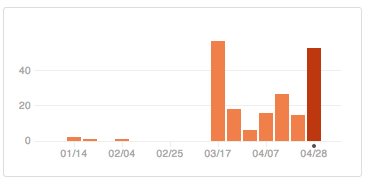
\includegraphics[scale=.5]{history.png}
\caption{A graph showing the commit history of the project over the course of the semester.}
\end{figure}

\begin{figure}[H]
\centering
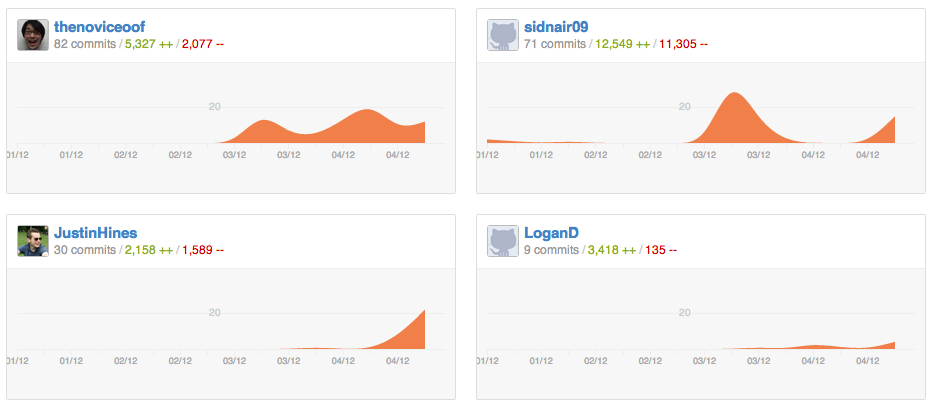
\includegraphics[width=\textwidth]{Contribution.png}
\caption{Diagram of Contributions to the Project. thenoviceof is Nathan, sidnair09 is Sid, JustinHines is Justin and Andrew since their pair program together and LoganD is Logan.}
\end{figure}


\part{Language Evolution}
Language Guru - Sid

\section{Language Changes}
The LRM changed very little during the course of our implementation. This is
because we were cautious when writing the LRM and anticipated that features we
thought would be simple might end up being difficult to implement. In fact, our
LRM did not require any parallelism in a DotPar compiler implementation. This is
because the language could conceivably be run in an environment in which
parallelism is infeasible or undesirable; adding unnecessary restrictions on the
compiler writer seemed imprudent.

The biggest issue we we came across was dealing with overloading. For instance,
we wanted to overload the \verb$map$ function, but support neither function
overloading nor inheritance. Thus, we could not support using \verb$map$ on an
array of numbers and an array of strings, for example. To solve this, we
introduced an \verb$Any$ type which can be used for built-in functions. This
maintains the paradigms of our type system, but means that it is possible to get
a type error after semantic analysis, which violates some definitions of static
typing.

Another feature on our wishlist that we wanted to implement but were forced to cut was Java
interoperability. Java interoperability would make our language practical in the
real world. Unfortunately, it would require generating an AST from bytecode in
order to do dependency analysis and to do type checking. That said, compiled
DotPar code can be used with Java code, just not the other way around.

\section{Implementing Parallelism}
Parallelization was another challenging feature. Because it is the selling
point of the language, we will briefly discuss the implementation details.
We decided that our focus would be data
parallelism on \verb$for$ loops and special constructs like the \verb$map$ and
\verb$reduce$ functions and list comprehensions. We did not want to parallelize
lines outside of blocks. This would require constructing a full data flow graph
and generating code that would wait for all dependencies to be computed
before executing a piece of code. While not infeasible, this introduced
additional complexity for minimal gain because the most expensive computations
tend to be in loops.

Due to time constraints, our analysis of data dependencies is limited to the
variable level. Thus, if each iteration of a loop from \verb$i$ to \verb$n$
writes to \verb$a[i]$ for some array \verb$a$, our code will think that there is
a dependence with between each iteration of these loops. This is known as a
\emph{false dependency}. Although every correct dependency analysis program
provably must generates some false dependencies, many common cases can be
optimized. There are well-known tests for array dependencies such as the
Banerjee GCD test and the Delta test. Because these tests are well-known and our
language provides ways to naturally parallelize maps and reduces even without
this analysis we decided not to implement these tests.

First, we call a function that has side effects \emph{impure}.  Since we only
parallelize maps, reduces, and list comprehensions, the only functions which are
impure are ones that make assignments to variables outside their immediate
scope.

Detecting associativity of functions is more difficult. Detecting it in the
general case is an open problem in the field. Without detecting these
properties, however, it becomes impossible to parallelize certain classes of
problems. For instance, to parallelize a \verb$reduce$, the reduction function
must be associative. Fortunately, we are able to detect simple instances of
associativity, such as a \verb$sum$ or \verb$product$ function.

Thus, though we do miss some opportunities for parallelism, we also never
incorrectly detect an opportunity for parallelism, so DotPar does not introduce
race conditions.

\section{Language Implementation Tools}
To implement the language, we wrote the compiler in OCaml and used Scala as our
target language.

We used OCaml because we wanted to learn a functional paradigm. OCaml is also
often used for writing compilers, so many relevant tools and resources are
available. We used \verb$ocamllex$ and \verb$ocamlyacc$ for lexing and parsing,
respectively. The tools are similar to \verb$lex$ and \verb$yacc$, but have
slightly different syntax that is more fitting for OCaml.

We compiled down to Scala for several reasons. First, it gives us first-class
functions and closures for free. If we compiled down to something like Java,
implementing closures would involve creating wrapper classes for functions to
make them first-class and wrapping scopes in objects to implement closures.
Second, it was more natural to compile our imperative constructs into Scala than
it would have been to compile it to a functional language like Haskell or even a
multiparadigm language like OCaml, which errs towards the functional.
Additionally, Scala is threaded, and allows us to have more granular control
over parallelism than a language like JavaScript. Furthermore, Scala is
statically and strongly typed. Since our language does some type checking and
requires types to be specified, it makes sense to use a language that makes use
of these constructs since statically typed language tend to be faster than
dynamically typed languages. Finally, Scala runs on the JVM\@. While this was not
as essential as the other requirements, it is nice that any code that runs on
the JVM will be able to use compiled DotPar code. In the future, we could
leverage the virtual machine to use other code that runs on the JVM in DotPar
code.

We require no unusual libraries. An OCaml compiler, \verb$ocamlyacc$,
\verb$ocamllex$, and Scala 2.9 or greater must be installed.

In order to keep the LRM and compiler consistent, we followed agile development
practices and had quick iterations that conformed to the language spec. We also
kept track of the features we had left to implement using GitHub. This is
explain in more detail in Part IV, Section 18.2.


\part{Translator Architecture}
System Architect - Justin
\section{Block Diagram}
\begin{figure}[H]
\centering
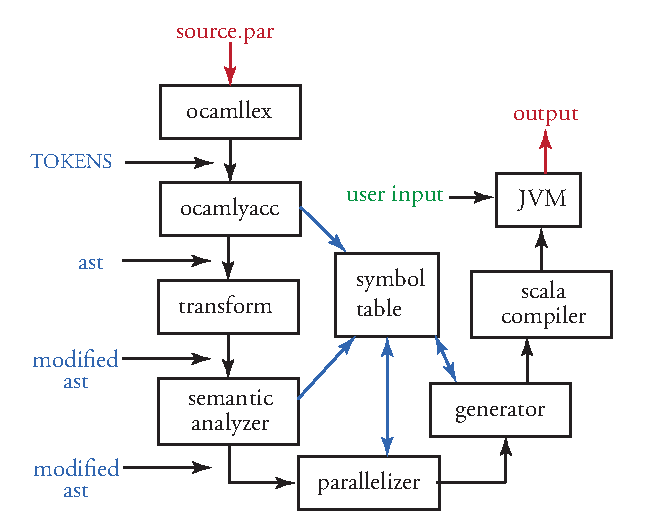
\includegraphics[scale=1]{blockdiagram.eps} 
\caption{Block Diagram of the DotPar compiler.}
\end{figure}

\section{Interfaces}
Dotpars interface, as seen above follows a standard form of a compiler. The raw
source file is fed into the \verb=lexer=, \verb=ocamllex=, which outputs a series of tokens that is then
parsed by \verb=ocamlyacc=.  \verb=Ocamlyacc= uses a our custom type system to output an abstract
syntax tree.

Our abstract syntax tree then undergoes a series of modifications and optimizations before it
is complied down into scala and fed into the scala compiler.  The first transform
is done by the aptly named \verb=transform.ml= which reverses nodes with a tree.  The lexer
recurses right to left, and thus all lists are stored backeds and need to be reversed.
The transform outputs a modified AST which is then fed into the semantic analyzer.

The semantic analyzer performs an extensive amount of type checking, making 
sense of a user's source code, throwing errors where need be, recovering from 
small errors if possible,  and adding necessary information to the symbol table.  

Next, the parallelizer, in which the main optimizations are performed, takes
the modified AST from the semantic analyzer. The first pass
performs a series of tests to find, and declare certain functions as
\emph{pure}. A second pass marks certain functions as \emph{associative}.
These functions that are pure can be parallelized in maps and list
comprehensions, and pure and associative functions can be parallelized in
reduces as well. Our optimizatinos focus on major bottlenecks of source programs
including maps, reduces, and list comprehensions.

Lastly, the parallelizer outputs a modified AST which is fed into the generator, 
which does a pass over the ast, translating the tree into and creating parallelized 
functions where applicable, which is lastly fed into the scala compiler.  The
scala compiler then complies down the JVM which can then be run on a target machine.

Dotpar uses a total of 5 different passes over the abstract syntax, performing 
checks and optimizations at each state to insure relability.  With this comes
the added benefit of a program not required to be parallizable to be run.  Dotpar
will only attempt to parallelize a program after extensive checks which gives add 
compile security and relability.

\section{Implementation}
The original grammar, written using \verb=yacc= and \verb=lex=, was designed and
implemented Sid Nair and Nathan Hwang. The conversion to OCaml was done by Sid
Nair and Justin Hines. The parsing to create the AST was was completed by
Nathan Hwang and Justin Hines. An additional transformation pass on the tree was
done by Nathan Hwang. The semantic analysis pass was implemented by Justin
Hines and Andrew Hitti. The parallelizer was implemented by Sid Nair with minor
contributions from Justin Hines and Nathan Hwang. The Generator was implemented
by Nathan Hwang with signifcant contributions from Sid Nair, Andrew Hitti, and
Justin Hines. Test cases were written by all group members, but the primary
contributors were Nathan Hwang, Andrew Hitti, and Logan Donovan.


\part{Development and Run-time Environment}
System Integrator - Nathan

\section{Development Environment}

In order to effectively develop the Dotpar compiler, we used standard
development tools to streamline our development cycle, ensure a
consistent build across platforms, and generate binaries from Dotpar
code.

\subsection{Compiler Build Process}

We used a Makefile to manage our build and testing process, relying on
this standard tool in the open source world to abstract away the act
of building the compiler anew.

Holding with tradition, the Makefile provides familiar commands such
as \texttt{all}, \texttt{clean}, and \texttt{test}, which each in turn
generate a binary, clean up generated intermediate files, and run the
test suites on the generated binary, respectively. We reference our
Makefile in figure \ref{makefile}.

\begin{figure}[H]
\begin{verbatim}
SRC = src
OCAML_PATH = $(SRC)/ocaml

all: bin compiler

bin:
	mkdir bin

compiler:
	cd $(OCAML_PATH); \
	ocamlc -c ast.ml; \
	ocamlc -c transform.ml; \
	ocamlyacc parser.mly; \
	ocamlc -c parser.mli; \
	ocamllex scanner.mll; \
	ocamlc -c scanner.ml; \
	ocamlc -c parser.ml; \
	ocamlc -c semantic.ml; \
	ocamlc -c parallelizer.ml; \
	ocamlc -c generate.ml; \
	ocamlc -c compile.ml; \
	ocamlc -c dotpar.ml; \
	ocamlc -o ../../bin/dotpar scanner.cmo ast.cmo transform.cmo \
			parser.cmo semantic.cmo parallelizer.cmo generate.cmo compile.cmo \
			dotpar.cmo

clean_ocaml:
	rm -f bin/dotpar
	cd $(OCAML_PATH); \
	rm -f *.cmo scanner.ml parser.ml parser.mli *.cmi

test: parser_test semantic_test full_test

parser_test: compiler
	python tests/parser_test.py
semantic_test: compiler
	python tests/semantic_test.py
full_test: compiler
	scala tests/full_test.scala

clean: clean_ocaml

.PHONY: all compiler test clean
\end{verbatim}
\caption{Makefile for the project}
\label{makefile}
\end{figure}

Additionally, we provide a finer-grained access to our test suites
with such commands as \texttt{parser\_test}, \texttt{semantic\_test},
and \texttt{full\_test} which run the seperate test suites that target
the major parts of our compiler in turn. The test suites themselves
are detailed in the ``Testing Methodology'' section.

To manage the code and facilitate collaboration, we used a source
control system known as git, which has recently become a popular tool,
especially in the open source world. In particular, we extensively
used branches in order to allow development in different areas at the
same time. Also, we leveraged the excellent git hosting tool
github.com, as detailed in the ``Github'' section.

The \texttt{dotpar} compiler itself is built on OCaml, as detailed in
``Language Implementation Tools''. We invoke the OCaml compiler from
our Makefile, compiling each separate part of the compiler with
\texttt{ocamlc -c} and then linking them together with \texttt{ocamlc
  -o} in discrete steps. The compiler itself has no dependencies on
external OCaml libraries that are not packaged with the standard OCaml
environment, which enhances it's portability.

\subsection{Compilation Process}

The process of actually creating a binary from the generated compiler
is facilitated by a different program, a shell script named
\texttt{dotparc}. While \texttt{dotpar} takes Dotpar source code and
generates Scala code, \texttt{dotparc} reads in Dotpar files, runs
them through \texttt{dotpar}, and compiles the resulting Scala code to
an executable jar file. It does this by invoking the Scala compiler
\texttt{scalac} on the output Scala code, and packing the
\texttt{class} files into a jar along with the requisite Scala and
Dotpar support libraries. Then this jar is ready to be run on a JVM.

\subsection{Editor Plugins}

In order to facilitate writing tests, we wrote plugins for the popular
Vim and Emacs text editors to do code highlighting and indentation for
Dotpar files.

\subsection{Runtime Environment}

Our run-time is based on the JVM, as we leverage Scala, which compiles
down to JVM bytecode. More specifically, the generated JVM bytecode
relies on the included support Scala library files: without these, the
program will not run as compiled by \texttt{scalac}.

Finally, we include some supporting Scala code specifically tailored
to enabling our generated Dotpar code to run by extending the behavior
of the JVM and Scala runtimes to provide the semantics required by the
DotPar code.


\part{Test Plan}
System Tester - Andrew

\section{Testing Methodology}
For Dotpar we followed a very strict Test Driven Development plan. The
tests for both our parser and semantic analyzer were written weeks
before either was implemented. To begin thinking
about how to design a comprehensive test suite I began with my
IDE. Since Dotpar is a typed, compiled language I figured the warnings
and errors an IDE like Eclipse throws for Java would also pertain to
our language. After that initial round of tests, I walked through the
sample programs in our whitepaper and LRM to ensure they were
present in the test suite. I also created variations of each of
them that should either pass or fail.

Nathan and I pair programmed two python scripts,
\verb=parser_test.py= and \verb=semantic_test.py=, that contained our
tests with a table of contents at the top to allow for a high level
view of our test cases. It also gives us the ability to run them through our compiler and spit out each test that went wrong with its intended
behavior. This bit of optimization was extremely helpful! With a
single command, \verb=make semantic\_test=, we were able to compile all our
sources and run the python script that told us what it was supposed to
do.

In addition to the test cases, when Justin and I were writing the
semantic analyzer, he had the idea to add debug statements that
would print out which portion of code was running on which values. So,
when we fed a single test into our compiler it would spit out what is
was doing, adding to the symbol table, checking types, checking jump
statements, etc.. We could then trace whether or not we were
wrapping array accesses in their proper types and comparing nested
types correctly.

We also created a make \emph{full\_test} that compiles a series of
test programs written in Dotpar and compares them to scala
equivalents. This ensures that our code generation matches expected
scala output.  Overall, it was very helpful to think of test cases in
terms of pairs, a situation in which something should pass and a
situation in which it should not. So, for every concept, like brace
matching, type checking, comment nesting, etc. we would ensure that
there were variants of each that were supposed to be correct and
supposed to be incorrect. This was very helpful because sometimes our
analyzer would fail tests that were supposed to fail but for the wrong
reasons, or just fail everything so it looked like half our tests
passed but in reality only for the shallow reason that nothing really
worked.

\section{Test Programs}
Sample test cases:
\begin{verbatim}
func main:void() {
func fizzBuzz:void() {
  char[] fb = "FizzBuzz";
  char[] f = "Fizz";
  char[] b = "Buzz";
  for (number i = 1; i < 101; i = i + 1){
    if (i % 15 == 0){
      println(fb);
    } elif(i % 3 == 0) {
      println(f);
    } elif(i % 5 == 0) {
      println(b);
    } else {
      println(i);
    }
  }
}
}

func main:void() {
func fib:number(number n) {
  if (n == 0) {
    return 0;
  }
  elif (n == 1) {
    return 1;
  } else {
    return fib(n-1) + fib(n-2);
  } 
}
}

func main:void() {
  number[] xx = [1, 2];
  number[] yy = [1, 2];
  [x*y for number x, number y in xx,yy if (x==1)];
}

\end{verbatim}


\part{Conclusions}
\section{Group Lessons and Advice for Future Groups}
\subsection{Starting Early}
\subsection{Work Must be Done Eventually}
\subsection{Make Group Deadlines Hard Deadlines}
\section{Individual Lessons}
\subsection{Logan - Have a Backup Plan}
We started off the semester with a great group of individuals who are all capable and motivated. We were able to assign appropriate roles based on each member's skillset and what they wanted to do. Even with that, you have to count on things going wrong. I didn’t plan on getting very sick for over a month or having to miss a week and a half of school. The biggest problem was that it made it hard to communicate with the team and help coordinate who was taking over my responsibilities temporarily. Nathan really stepped up and helped keep the group on track with our schedule. I could have also been better about following up when people couldn’t make meetings due to other commitments. Occasionally, it would be the next weekly meeting before I got caught up on their progress. 

\subsection{Sid}
\subsection{Justin - Don't Be Afraid to Ask for Help}

\subsection{Andrew - Pair Programming}
Pair programming is fun and helpful. When we worked in pairs on one computer we wrote better code, faster. Having two sets of eyes looking out for syntax errors and keeping logic consistent went a very long way in helping to reduce bugs and accomplish tasks in a more timely fashion. I felt this was helpful especially in the beginning when we were all learning ocaml because I would remember some syntax and functions and my partner would remember others. In this respect, we were able to learn from each other. The knowledge transfer experience contributed to the cohesion of our group.

\subsection{Nathan - Projects Will Take as Much Time as You Let Them}
I learned that no matter how ambitious or puny a project may seem at
first, the expectations and goals attached to that project can and
will grow and shrink as availability becomes more or less scarce: in
other words, projects will grow to fill the time allotted to them. We
originally envisioned the project being functionally done a week
before it was due, but since we had that buffer time, why not use it?
And now here we are, pushing this up to the last minute. This lesson
can also be known as ``self discipline is hard''.

\section{Advice for Future Groups}

\section{Ideas for Improving the Course}
\
Example timeline for completion of steps
Having deadlines for individual parts of the compiler
I feel it might even be beneficial for the class to implement advised deadlines for groups that would recommend implementing this aspect of the compiler by this date.
More indepth discussion of implementation tools


\part{Appendix}
Include a listing of the complete source code with identification of
who wrote which module of the compiler. This listing does not have to
be included in the paper copy of the final report.


\end{document}
